\documentclass{article}
\usepackage[english]{babel}
\usepackage[letterpaper,top=2cm,bottom=2cm,left=3cm,right=3cm,marginparwidth=1.75cm]{geometry}
\usepackage{amsmath}
\usepackage{graphicx}
\usepackage[colorlinks=true, allcolors=blue]{hyperref}
\usepackage[numbers]{natbib}
\usepackage{listings}

\title{NOvA Production 6 Validation Task Force Contribution Summary}
\author{Hanyi Chen}

\begin{document}
\maketitle

\section{$\nu_e$ ND MC/MC}

For the vertex and shower-start/stop position variables, the Prod~6/Prod~5.1 ratios are mostly flat after requiring true vertex containment and $N_{\rm hit}\geq 15$. The $N_{\rm hit}\geq 15$ requirement was applied to make the Prod~5.1 sample more comparable to Prod~6, where the pixel-map requirement removes slices with fewer than 15 hits. The remaining differences are mostly outside the fiducial and containment cut regions.

The slice $N_{\rm hit}$ distribution in true fiducial volume after the quality, fiducial, and containment cuts is shown in Figure~\ref{fig:nhit-nd-mc}. Two features are visible: a kink near the 15--30 hit region, and a broad shoulder-like shape difference around 50--120 hits. The first feature was checked at other cut levels and is attributed to the unretuned fiducial and containment cuts. The second feature was later compared against data/data and appears to be driven by a simulation-level difference rather than a reconstruction effect.

\begin{figure}[htbp]
    \centering
    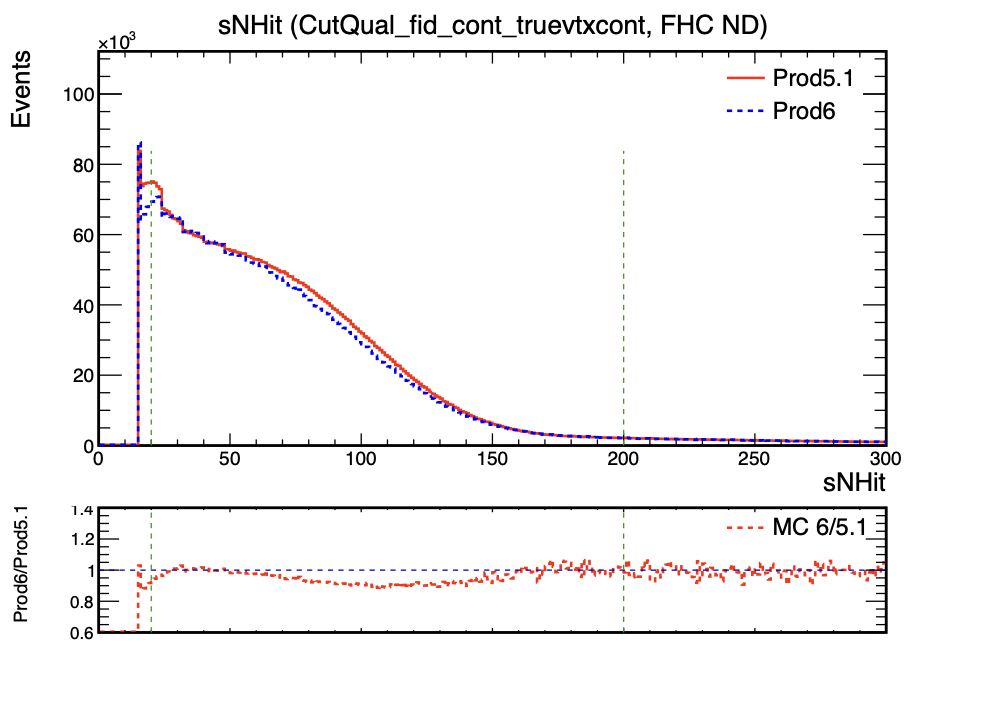
\includegraphics[width=0.6\textwidth,trim={0cm 2.5cm 0cm 0cm},clip]{images-hchen/nhit_ND_MC.png}
    \caption{\small Slice $N_{\rm hit}$ distribution in the ND MC comparison after the quality, fiducial, and containment cuts.~\cite{mc-vali-1}}
    \label{fig:nhit-nd-mc}
\end{figure}

The longest-prong distribution is shifted toward shorter lengths in Prod~6, as shown in Figure~\ref{fig:longestProng-nd-mc}. The true-channel breakdown indicates that this shift is mainly associated with $\nu_\mu$ CC events.

\begin{figure}[htbp]
    \centering
    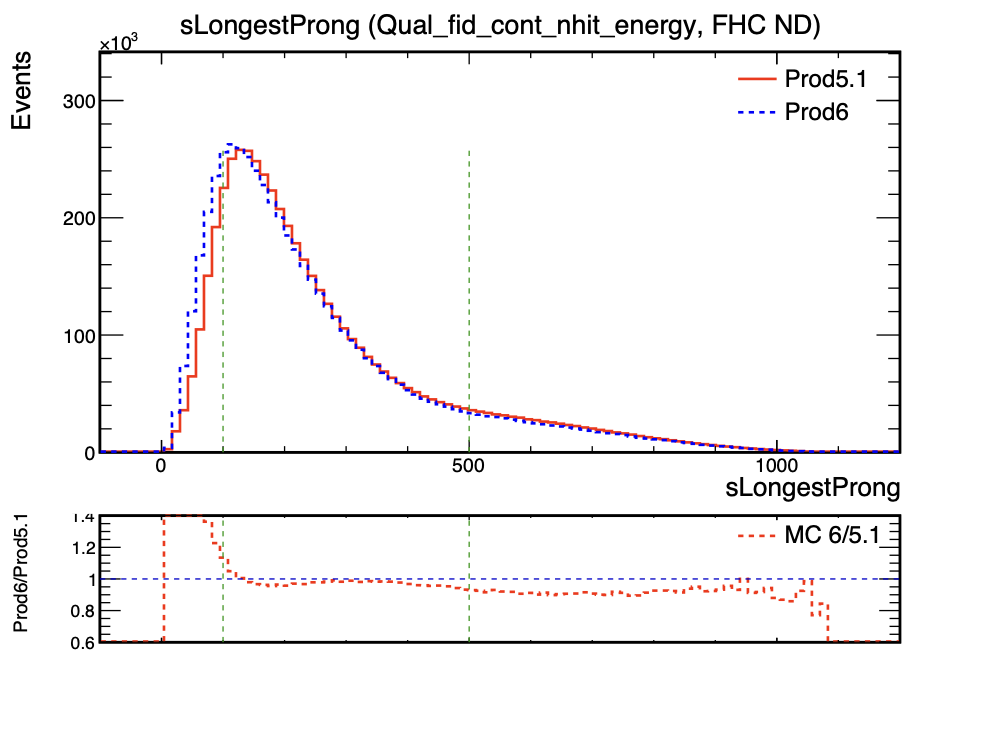
\includegraphics[width=0.6\textwidth,trim={0cm 2.5cm 0cm 0cm},clip]{images-hchen/longest_prong_MC_ND.png}
    \caption{\small Longest-prong distribution in the ND MC comparison, after applying the ND $\nu_e$ preselection except for the longest-prong cut itself.~\cite{mc-vali-1}}
    \label{fig:longestProng-nd-mc}
\end{figure}

These preselection-variable differences lead to a reduction in the selected event rate after the $\nu_e$ preselection. In particular, the fiducial and containment cuts reduce the Prod~6/Prod~5.1 ratio because the cut values have not yet been retuned for Prod~6. The longest-prong cut also contributes to a lower Prod~6/Prod~5.1 ratio at lower energy.

For the PID selection, Prod~6 and Prod~5.1 were compared using a matched-efficiency approach. The Prod~6 PID threshold was adjusted so that the signal efficiency after preselection matched the Prod~5.1 value:
\[
\frac{N_{\rm sig}({\rm full~selection}\mid{\rm Prod~5.1})}
     {N_{\rm sig}({\rm preselection}\mid{\rm Prod~5.1})}
=
\frac{N_{\rm sig}({\rm full~selection}\mid{\rm Prod~6})}
     {N_{\rm sig}({\rm preselection}\mid{\rm Prod~6})}.
\]
Here the signal is defined as $\nu_e$ in FHC and $\bar{\nu}_e$ in RHC.

After applying the matched-efficiency PID selection, Prod~6 still shows an overall reduction in efficiency and purity relative to Prod~5.1~\cite{mc-vali-2}. Part of the difference is due to the preselection variables and the lack of retuning of the preselection cuts. Another contribution comes from the different behavior of the Transformer CVN relative to the previous CVN. In the ND $\nu_e$ sample, the true-channel comparison in Figure~\ref{fig:pid_truech} suggests that the Transformer CVN rejects $\nu_\mu$ CC background more efficiently, but is less effective at rejecting NC background.

\begin{figure}[htbp]
    \centering
    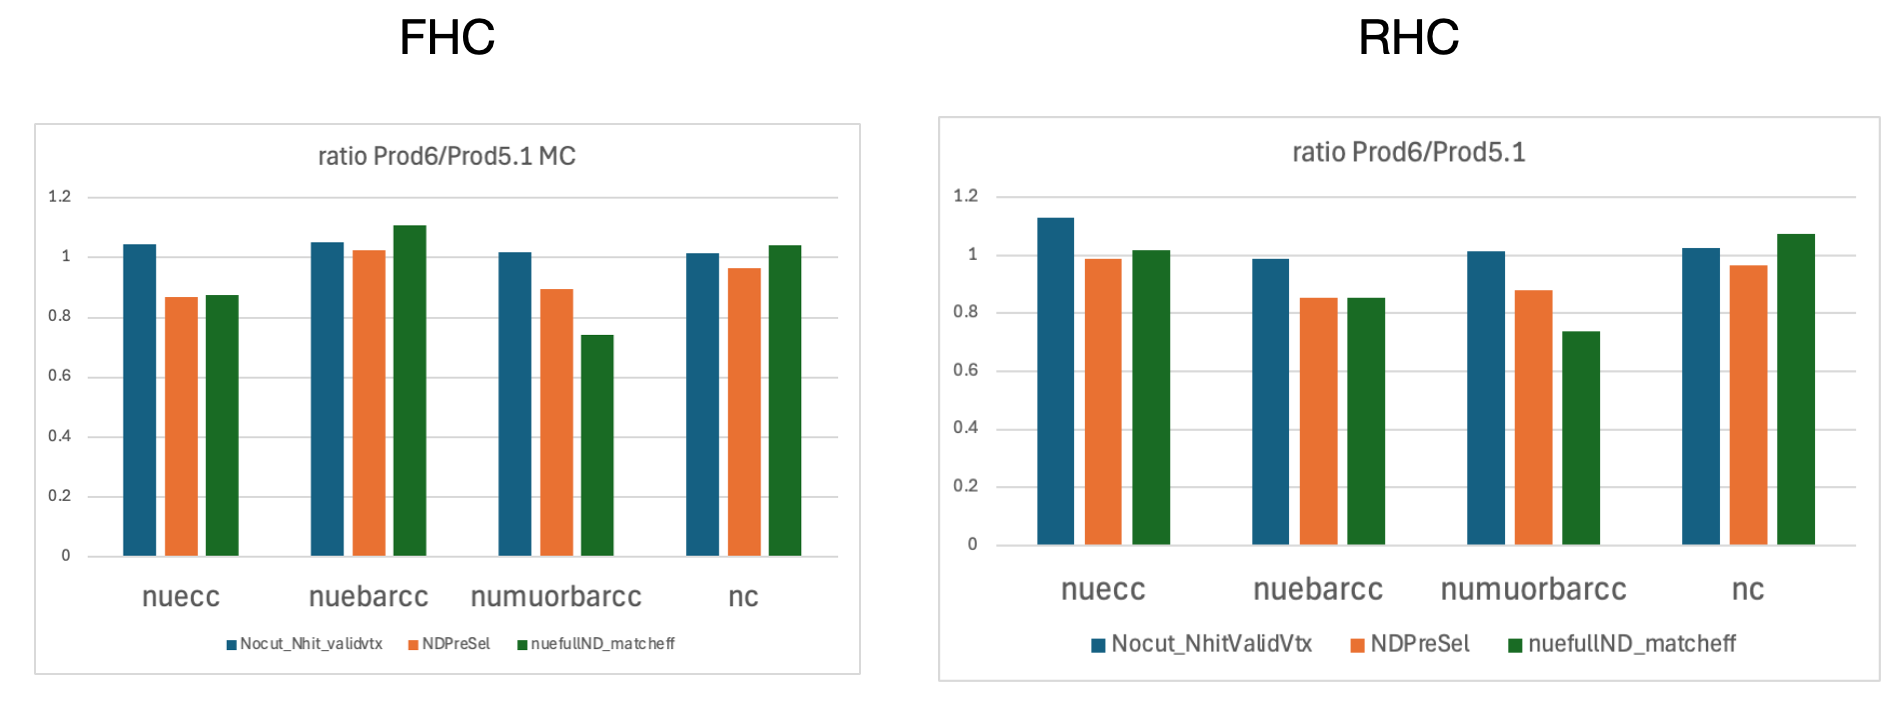
\includegraphics[width=0.99\textwidth,trim={0cm 0cm 0cm 0cm},clip]{images-hchen/pid_truech.png}
    \caption{\small Ratio of the Prod~6 event count to the Prod~5.1 event count at three selection stages. Blue shows the sample with only the valid-vertex and $N_{\rm hit}\geq 15$ requirements, orange shows the $\nu_e$ preselection, and green shows the full ND $\nu_e$ selection with matched PID efficiency.~\cite{data-vali}}
    \label{fig:pid_truech}
\end{figure}

\section{$\nu_e$ ND Data/Data}

The ND data/data comparison was performed using run/subrun-matched Prod~5.1 and Prod~6 data samples~\cite{data-vali-numu}. The validation focused on slice-level variables after requiring a valid vertex and $N_{\rm hit}\geq 15$, after the ND $\nu_e$ preselection, and after the full selection using the Prod~6 PID thresholds obtained from the ND MC/MC matched-efficiency study.

The position-related variables, including reconstructed vertex position, slice min/max coordinates, and shower start/stop positions, show broadly consistent behavior between Prod~5.1 and Prod~6. This is also consistent with the corresponding MC/MC comparison.

The main differences are observed in slice $N_{\rm hit}$, slice calorimetric energy, and longest-prong length. After the PID selection, Prod~6 data shows an excess at higher values of these variables compared to Prod~5.1. One example using slice calorimetric energy is shown in Figure~\ref{fig:calE}. This trend is not seen in the MC/MC comparison. For slice calorimetric energy, the low-energy discrepancy appears to be connected to the $N_{\rm hit}$ cut, the longest-prong cut, and the PID selection, while the higher-energy discrepancy is mostly introduced by the PID selection.

\begin{figure}[htbp]
    \centering
    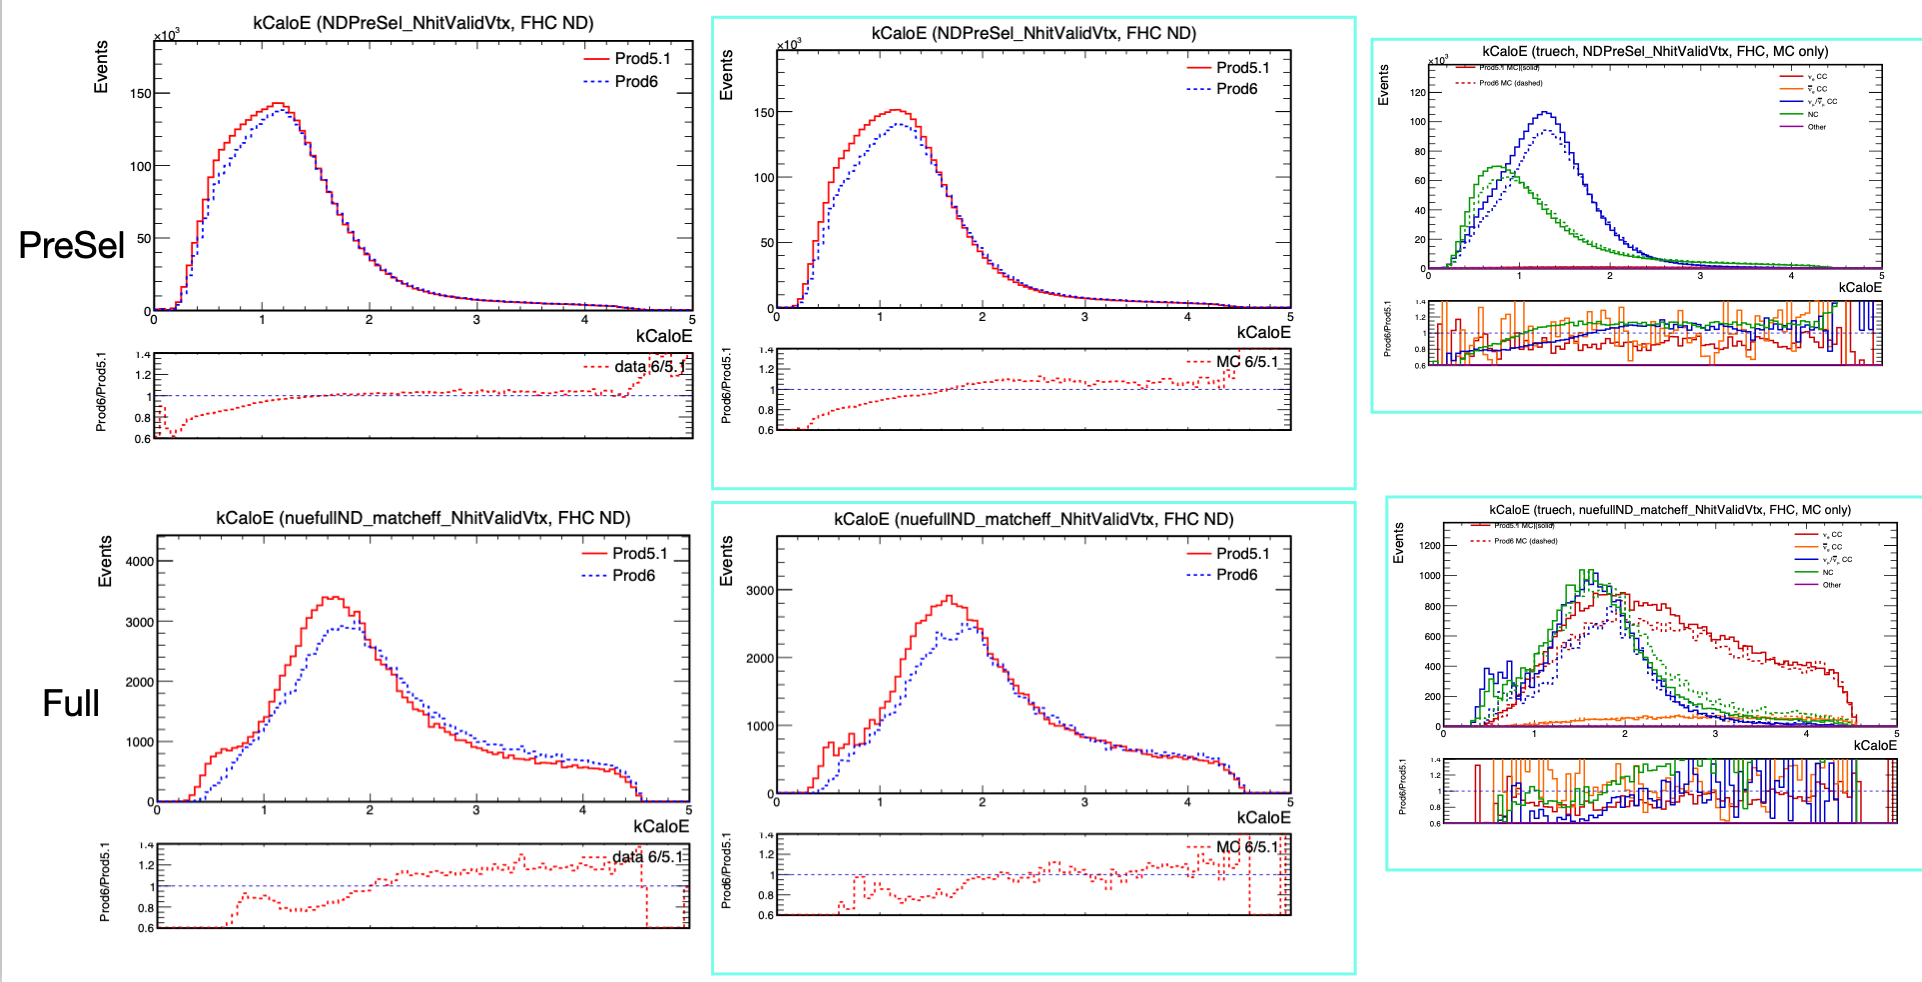
\includegraphics[width=0.99\textwidth,trim={0.1cm 0cm 0cm 0cm},clip]{images-hchen/calE_data.png}
    \caption{\small Calorimetric energy in a slice. The upper row is at the $\nu_e$ preselection level, and the bottom row is at the full matched-efficiency selection level. The plots with blue frames show MC, while those without blue frames show data.~\cite{data-vali}}
    \label{fig:calE}
\end{figure}

The PID-selection behavior in data/data is therefore somewhat different from the MC/MC expectation, as shown in Figure~\ref{fig:pid_dataMC}. Differences in the signal/background composition of the PID-selected data sample relative to MC may be one explanation for this difference.

\begin{figure}[htbp]
    \centering
    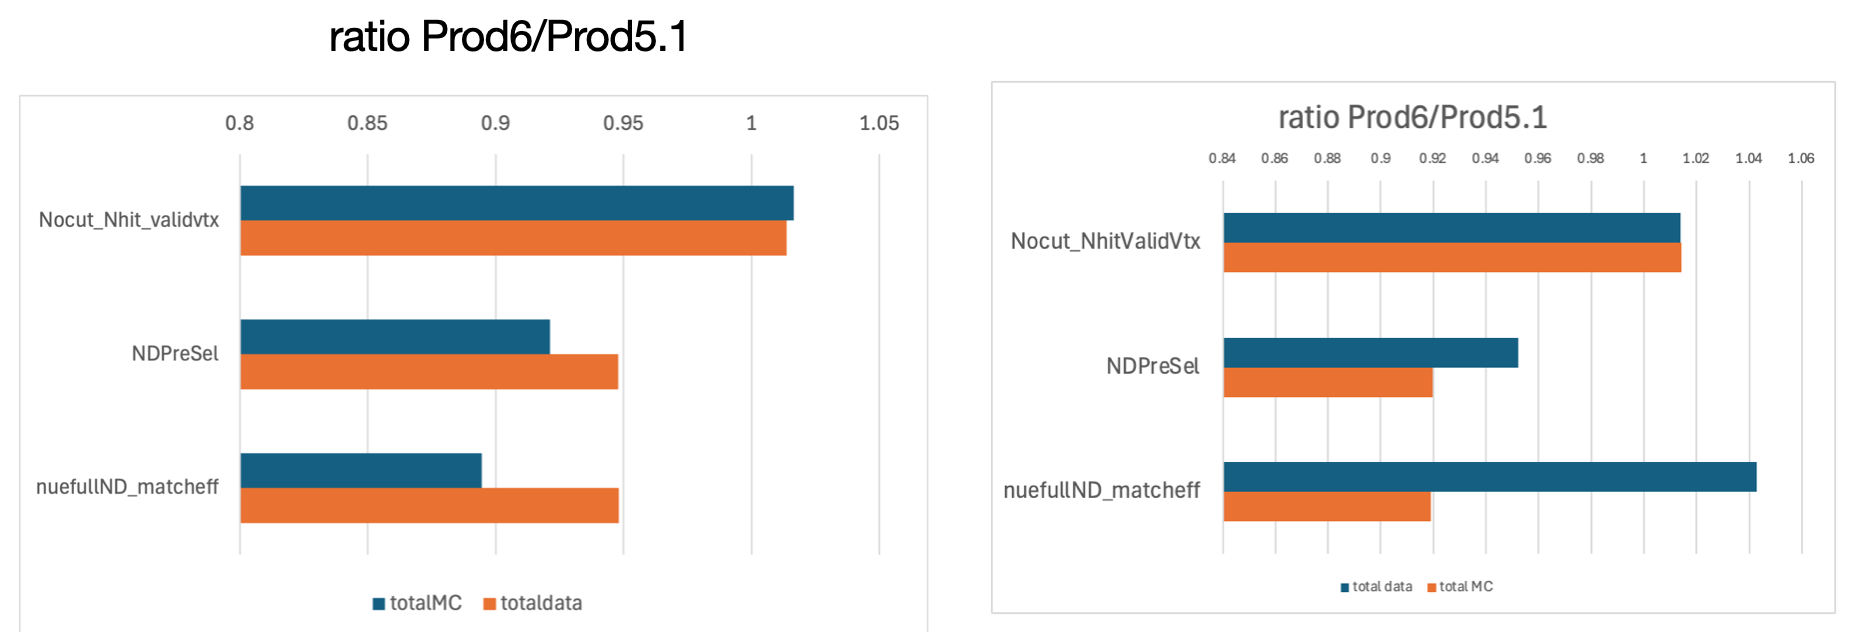
\includegraphics[width=0.99\textwidth,trim={0cm 0cm 0cm 0cm},clip]{images-hchen/pid_dataMC.png}
    \caption{\small Ratio of the Prod~6 event count to the Prod~5.1 event count at three selection stages. Blue shows MC and orange shows data.~\cite{data-vali}}
    \label{fig:pid_dataMC}
\end{figure}



\bibliographystyle{unsrtnat}
\bibliography{summary-hchen}

\end{document}